%%%%%%%%%%%%%%%%%%%%%%%%%%%%%%%%%%%%%%%%
% Classicthesis Typographic Thesis
% LaTeX Template
% Version 1.3 (15/2/14)
%
% This template has been downloaded from:
% http://www.LaTeXTemplates.com
%
% Original author:
% André Miede (http://www.miede.de)
%
% License:
% CC BY-NC-SA 3.0 (http://creativecommons.org/licenses/by-nc-sa/3.0/)
%
% General Tips:
% 1) Make sure to edit the classicthesis-config.file
% 2) New enumeration (A., B., C., etc in small caps): \begin{aenumerate} \end{aenumerate}
% 3) For margin notes: \marginpar or \graffito{}
% 4) Do not use bold fonts in this style, it is designed around them
% 5) Use tables as in the examples
% 6) See classicthesis-preamble.sty for useful commands
%
%%%%%%%%%%%%%%%%%%%%%%%%%%%%%%%%%%%%%%%%%

%----------------------------------------------------------------------------------------
%	PACKAGES AND OTHER DOCUMENT CONFIGURATIONS
%----------------------------------------------------------------------------------------

\documentclass[
		twoside,openright,titlepage,numbers=noenddot,headinclude,%1headlines,
                footinclude=true,cleardoublepage=empty,
                BCOR=5mm,paper=a4,fontsize=11pt, % Binding correction, paper type and font size
                ngerman,american, % Languages
                ]{scrreprt}

% Includes the file which contains all the document configurations and packages - make sure to edit this file
%%%%%%%%%%%%%%%%%%%%%%%%%%%%%%%%%%%%%%%%%
% Thesis Configuration File
%
% The main lines to change in this file are in the DOCUMENT VARIABLES
% section, the rest of the file is for advanced configuration.
%
%%%%%%%%%%%%%%%%%%%%%%%%%%%%%%%%%%%%%%%%%

%----------------------------------------------------------------------------------------
%	DOCUMENT VARIABLES
%	Fill in the lines below to enter your information into the thesis template
%	Each of the commands can be cited anywhere in the thesis
%----------------------------------------------------------------------------------------

% Remove drafting to get rid of the '[ Date - classicthesis version 4.0 ]' text at the bottom of every page
\PassOptionsToPackage{eulerchapternumbers,listings,drafting, pdfspacing, subfig,beramono,eulermath,parts}{classicthesis}
% Available options: drafting parts nochapters linedheaders eulerchapternumbers beramono eulermath pdfspacing minionprospacing tocaligned dottedtoc manychapters listings floatperchapter subfig
% Adding 'dottedtoc' will make page numbers in the table of contents flushed right with dots leading to them

\newcommand{\myTitle}{Titel meiner Abschlu\ss arbeit}
\newcommand{\mySubtitle}{Arbeit zur Erlangung des Titels Bachelor of Science}
\newcommand{\myName}{Tim Michael Jagodzinski\xspace}
\newcommand{\myProf}{Prof. Dr. Targo Pavlista\xspace}
\newcommand{\myFaculty}{Fachbereich VI, Informatik und Medien\xspace}
\newcommand{\myUni}{Beuth Hochschule für Technik Berlin\xspace}
\newcommand{\myLocation}{Berlin\xspace}
\newcommand{\myTime}{M\"{a}rz 2015\xspace}
\newcommand{\myVersion}{Version 0.0\xspace}

%----------------------------------------------------------------------------------------
%	USEFUL COMMANDS
%----------------------------------------------------------------------------------------

\newcommand{\ie}{i.\,e.}
\newcommand{\Ie}{I.\,e.}
\newcommand{\eg}{e.\,g.}
\newcommand{\Eg}{E.\,g.}

\newcounter{dummy} % Necessary for correct hyperlinks (to index, bib, etc.)
\providecommand{\mLyX}{L\kern-.1667em\lower.25em\hbox{Y}\kern-.125emX\@}

%----------------------------------------------------------------------------------------
%	PACKAGES
%----------------------------------------------------------------------------------------

\usepackage{lipsum} % Used for inserting dummy 'Lorem ipsum' text into the template

%------------------------------------------------

\PassOptionsToPackage{utf8}{inputenc} % latin9 (ISO-8859-9) = latin1+"Euro sign"
\usepackage{inputenc}

 %------------------------------------------------

%\PassOptionsToPackage{ngerman,american}{babel}  % Change this to your language(s)
% Spanish languages need extra options in order to work with this template
%\PassOptionsToPackage{spanish,es-lcroman}{babel}
\usepackage{babel}

%------------------------------------------------

\PassOptionsToPackage{square,numbers}{natbib}
 \usepackage{natbib}

 %------------------------------------------------

\PassOptionsToPackage{fleqn}{amsmath} % Math environments and more by the AMS
 \usepackage{amsmath}

 %------------------------------------------------

\PassOptionsToPackage{T1}{fontenc} % T2A for cyrillics
\usepackage{fontenc}

%------------------------------------------------

\usepackage{xspace} % To get the spacing after macros right

%------------------------------------------------

\usepackage{mparhack} % To get marginpar right

%------------------------------------------------

\usepackage{fixltx2e} % Fixes some LaTeX stuff

%------------------------------------------------

\PassOptionsToPackage{smaller}{acronym} % Include printonlyused in the first bracket to only show acronyms used in the text
\usepackage{acronym} % nice macros for handling all acronyms in the thesis

%------------------------------------------------

%\renewcommand*{\acsfont}[1]{\textssc{#1}} % For MinionPro
\renewcommand{\bflabel}[1]{{#1}\hfill} % Fix the list of acronyms

%------------------------------------------------

\PassOptionsToPackage{pdftex}{graphicx}
\usepackage{graphicx}

%----------------------------------------------------------------------------------------
%	FLOATS: TABLES, FIGURES AND CAPTIONS SETUP
%----------------------------------------------------------------------------------------

\usepackage{tabularx} % Better tables
\setlength{\extrarowheight}{3pt} % Increase table row height
\newcommand{\tableheadline}[1]{\multicolumn{1}{c}{\spacedlowsmallcaps{#1}}}
\newcommand{\myfloatalign}{\centering} % To be used with each float for alignment
\usepackage{caption}
\captionsetup{format=hang,font=small}
\usepackage{subfig}

%----------------------------------------------------------------------------------------
%	CODE LISTINGS SETUP
%----------------------------------------------------------------------------------------

\usepackage{listings}
%\lstset{emph={trueIndex,root},emphstyle=\color{BlueViolet}}%\underbar} % for special keywords
\lstset{language=[LaTeX]Tex, % Specify the language for listings here
keywordstyle=\color{RoyalBlue}, % Add \bfseries for bold
basicstyle=\small\ttfamily, % Makes listings a smaller font size and a different font
%identifierstyle=\color{NavyBlue}, % Color of text inside brackets
commentstyle=\color{Green}\ttfamily, % Color of comments
stringstyle=\rmfamily, % Font type to use for strings
numbers=left, % Change left to none to remove line numbers
numberstyle=\scriptsize, % Font size of the line numbers
stepnumber=5, % Increment of line numbers
numbersep=8pt, % Distance of line numbers from code listing
showstringspaces=false, % Sets whether spaces in strings should appear underlined
breaklines=true, % Force the code to stay in the confines of the listing box
%frameround=ftff, % Uncomment for rounded frame
frame=single, % Frame border - none/leftline/topline/bottomline/lines/single/shadowbox/L
belowcaptionskip=.75\baselineskip % Space after the "Listing #: Desciption" text and the listing box
}

%----------------------------------------------------------------------------------------
%	HYPERREFERENCES
%----------------------------------------------------------------------------------------

\PassOptionsToPackage{pdftex,hyperfootnotes=false,pdfpagelabels}{hyperref}
\usepackage{hyperref}  % backref linktocpage pagebackref
\pdfcompresslevel=9
\pdfadjustspacing=1

\hypersetup{
% Uncomment the line below to remove all links (to references, figures, tables, etc)
%draft,
colorlinks=true, linktocpage=true, pdfstartpage=3, pdfstartview=FitV,
% Uncomment the line below if you want to have black links (e.g. for printing black and white)
%colorlinks=false, linktocpage=false, pdfborder={0 0 0}, pdfstartpage=3, pdfstartview=FitV,
breaklinks=true, pdfpagemode=UseNone, pageanchor=true, pdfpagemode=UseOutlines,
plainpages=false, bookmarksnumbered, bookmarksopen=true, bookmarksopenlevel=1,
hypertexnames=true, pdfhighlight=/O, urlcolor=webbrown, linkcolor=RoyalBlue, citecolor=webgreen,
%------------------------------------------------
% PDF file meta-information
pdftitle={\myTitle},
pdfauthor={\textcopyright\ \myName, \myUni, \myFaculty},
pdfsubject={},
pdfkeywords={},
pdfcreator={pdfLaTeX},
pdfproducer={LaTeX with hyperref and classicthesis}
%------------------------------------------------
}

%----------------------------------------------------------------------------------------
%	BACKREFERENCES
%----------------------------------------------------------------------------------------

\usepackage{ifthen} % Allows the user of the \ifthenelse command
\newboolean{enable-backrefs} % Variable to enable backrefs in the bibliography
\setboolean{enable-backrefs}{false} % Variable value: true or false

\newcommand{\backrefnotcitedstring}{\relax} % (Not cited.)
\newcommand{\backrefcitedsinglestring}[1]{(Cited on page~#1.)}
\newcommand{\backrefcitedmultistring}[1]{(Cited on pages~#1.)}
\ifthenelse{\boolean{enable-backrefs}} % If backrefs were enabled
{
\PassOptionsToPackage{hyperpageref}{backref}
\usepackage{backref} % to be loaded after hyperref package
\renewcommand{\backreftwosep}{ and~} % separate 2 pages
\renewcommand{\backreflastsep}{, and~} % separate last of longer list
\renewcommand*{\backref}[1]{}  % disable standard
\renewcommand*{\backrefalt}[4]{% detailed backref
\ifcase #1
\backrefnotcitedstring
\or
\backrefcitedsinglestring{#2}
\else
\backrefcitedmultistring{#2}
\fi}
}{\relax}

%----------------------------------------------------------------------------------------
%	AUTOREFERENCES SETUP
%	Redefines how references in text are prefaced for different
%	languages (e.g. "Section 1.2" or "section 1.2")
%----------------------------------------------------------------------------------------

\makeatletter
\@ifpackageloaded{babel}
{
\addto\extrasamerican{
\renewcommand*{\figureautorefname}{Figure}
\renewcommand*{\tableautorefname}{Table}
\renewcommand*{\partautorefname}{Part}
\renewcommand*{\chapterautorefname}{Chapter}
\renewcommand*{\sectionautorefname}{Section}
\renewcommand*{\subsectionautorefname}{Section}
\renewcommand*{\subsubsectionautorefname}{Section}
}
\addto\extrasngerman{
\renewcommand*{\paragraphautorefname}{Absatz}
\renewcommand*{\subparagraphautorefname}{Unterabsatz}
\renewcommand*{\footnoteautorefname}{Fu\"snote}
\renewcommand*{\FancyVerbLineautorefname}{Zeile}
\renewcommand*{\theoremautorefname}{Theorem}
\renewcommand*{\appendixautorefname}{Anhang}
\renewcommand*{\equationautorefname}{Gleichung}
\renewcommand*{\itemautorefname}{Punkt}
}
\providecommand{\subfigureautorefname}{\figureautorefname} % Fix to getting autorefs for subfigures right
}{\relax}
\makeatother

%----------------------------------------------------------------------------------------

\usepackage{classicthesis}

%----------------------------------------------------------------------------------------
%	CHANGING TEXT AREA
%----------------------------------------------------------------------------------------

%\linespread{1.05} % a bit more for Palatino
%\areaset[current]{312pt}{761pt} % 686 (factor 2.2) + 33 head + 42 head \the\footskip
%\setlength{\marginparwidth}{7em}%
%\setlength{\marginparsep}{2em}%

%----------------------------------------------------------------------------------------
%	USING DIFFERENT FONTS
%----------------------------------------------------------------------------------------

%\usepackage[oldstylenums]{kpfonts} % oldstyle notextcomp
%\usepackage[osf]{libertine}
%\usepackage{hfoldsty} % Computer Modern with osf
%\usepackage[light,condensed,math]{iwona}
%\renewcommand{\sfdefault}{iwona}
%\usepackage{lmodern} % <-- no osf support :-(
%\usepackage[urw-garamond]{mathdesign} <-- no osf support :-(


\begin{document}

\frenchspacing % Reduces space after periods to make text more compact

\raggedbottom % Makes all pages the height of the text on that page

\selectlanguage{ngerman} % Select your default language - e.g. american or ngerman

%\renewcommand*{\bibname}{new name} % Uncomment to change the name of the bibliography
%\setbibpreamble{} % Uncomment to include a preamble to the bibliography - some text before the reference list starts

\pagenumbering{roman} % Roman page numbering prior to the start of the thesis content (i, ii, iii, etc)

\pagestyle{plain} % Suppress headers for the pre-content pages

%----------------------------------------------------------------------------------------
%	PRE-CONTENT THESIS PAGES
%----------------------------------------------------------------------------------------

% Title Page

\begin{titlepage}

\begin{addmargin}[-1cm]{-3cm}
\begin{center}
\large

\hfill
\vfill

\begingroup
\color{Maroon}\spacedallcaps{\myTitle} \\ \bigskip % Thesis title
\endgroup

\spacedlowsmallcaps{\myName} % Your name

\vfill


\includegraphics[width=6cm]{gfx/Beuth_Logo_basis.eps} \\ \bigskip % Picture

\mySubtitle \\ \medskip % Thesis subtitle
%\myDegree \\
%\myDepartment \\
\myFaculty \\
\myUni \\ \bigskip

\myTime\ -- \myVersion % Time and version

\vfill

\end{center}
\end{addmargin}

\end{titlepage}
 % Main title page

% Back of the title page

\thispagestyle{empty}

\hfill

\vfill

\noindent\myName: \textit{\myTitle,} \mySubtitle, an der Beuth-Hochschule f\"{u}r Technik zu Berlin.%\myDegree,
\textcopyright\ \myTime

% You may wish to do something with the back of the title page, such as including your supervisors, location or time frame of the work. Below is an example of doing so although you may want to tweak it to your liking.

%\bigskip

\noindent\spacedlowsmallcaps{Betreuer}: \\
\myProf \\
%\myOtherProf \\
\noindent\spacedlowsmallcaps{Gutachter}: \\
\mySupervisor

%\medskip \\

\noindent\spacedlowsmallcaps{Ort}: \\
\myLocation

%\medskip \\

%\noindent\spacedlowsmallcaps{Time Frame}: \\
%\myTime
 % Back of the title page

\cleardoublepage% Dedication

\thispagestyle{empty}
\refstepcounter{dummy}

\pdfbookmark[1]{Dedication}{Dedication} % Bookmark name visible in a PDF viewer

\vspace*{3cm}

\begin{center}
\emph{Ohana} means family. \\
Family means nobody gets left behind, or forgotten. \\ \medskip
--- Lilo \& Stitch
\end{center}

\medskip

\begin{center}
Dedicated to the loving memory of Rudolf Miede. \\ \smallskip
1939\,--\,2005
\end{center}
 % Dedication page

%\cleardoublepage\include{FrontBackMatter/Foreword} % Uncomment and create a Foreword.tex to include a foreword

\cleardoublepage% Abstract

\pdfbookmark[1]{Abstract}{Abstract} % Bookmark name visible in a PDF viewer

\begingroup
\let\clearpage\relax
\let\cleardoublepage\relax
\let\cleardoublepage\relax

\chapter*{Abstract} % Abstract name

Short summary of the contents\dots

\endgroup			

\vfill % Abstract page

%\cleardoublepage% Publications - a page listing research articles written using content in the thesis

\pdfbookmark[1]{Publications}{Publications} % Bookmark name visible in a PDF viewer

\chapter*{Publications} % Publications page text

Some ideas and figures have appeared previously in the following publications:

\bigskip

\noindent Put your publications from the thesis here. The packages \texttt{multibib} or \texttt{bibtopic} etc. can be used to handle multiple different bibliographies in your document.
 % Publications from the thesis page

%\cleardoublepage% Acknowledgements

\pdfbookmark[1]{Acknowledgements}{Acknowledgements} % Bookmark name visible in a PDF viewer

\begin{flushright}{\slshape    
We have seen that computer programming is an art, \\ 
because it applies accumulated knowledge to the world, \\ 
because it requires skill and ingenuity, and especially \\
because it produces objects of beauty.} \\ \medskip
--- \defcitealias{knuth:1974}{Donald E. Knuth}\citetalias{knuth:1974} \citep{knuth:1974}
\end{flushright}

\bigskip

%----------------------------------------------------------------------------------------

\begingroup

\let\clearpage\relax
\let\cleardoublepage\relax
\let\cleardoublepage\relax

\chapter*{Acknowledgements} % Acknowledgements section text

Put your acknowledgements here.\\

\noindent Many thanks to everybody who already sent me a postcard!\\

\noindent Regarding the typography and other help, many thanks go to Marco Kuhlmann, Philipp Lehman, Lothar Schlesier, Jim Young, Lorenzo Pantieri and Enrico Gregorio\footnote{Members of GuIT (Gruppo Italiano Utilizzatori di \TeX\ e \LaTeX )}, J\"org Sommer, Joachim K\"ostler, Daniel Gottschlag, Denis Aydin, Paride Legovini, Steffen Prochnow, Nicolas Repp, Hinrich Harms, Roland Winkler,  and the whole \LaTeX-community for support, ideas and some great software.

\bigskip

\noindent\emph{Regarding \mLyX}: The \mLyX\ port was intially done by
\emph{Nicholas Mariette} in March 2009 and continued by
\emph{Ivo Pletikosi\'c} in 2011. Thank you very much for your work and the contributions to the original style.

\endgroup % Acknowledgements page

\pagestyle{scrheadings} % Show chapter titles as headings

\cleardoublepage% Table of Contents - List of Tables/Figures/Listings and Acronyms

\refstepcounter{dummy}

\pdfbookmark[1]{\contentsname}{tableofcontents} % Bookmark name visible in a PDF viewer

\setcounter{tocdepth}{2} % Depth of sections to include in the table of contents - currently up to subsections

\setcounter{secnumdepth}{3} % Depth of sections to number in the text itself - currently up to subsubsections

\manualmark
\markboth{\spacedlowsmallcaps{\contentsname}}{\spacedlowsmallcaps{\contentsname}}
\tableofcontents
\automark[section]{chapter}
\renewcommand{\chaptermark}[1]{\markboth{\spacedlowsmallcaps{#1}}{\spacedlowsmallcaps{#1}}}
\renewcommand{\sectionmark}[1]{\markright{\thesection\enspace\spacedlowsmallcaps{#1}}}

\clearpage

\begingroup
\let\clearpage\relax
\let\cleardoublepage\relax
\let\cleardoublepage\relax

%----------------------------------------------------------------------------------------
%	List of Figures
%----------------------------------------------------------------------------------------

\refstepcounter{dummy}
%\addcontentsline{toc}{chapter}{\listfigurename} % Uncomment if you would like the list of figures to appear in the table of contents
\pdfbookmark[1]{\listfigurename}{lof} % Bookmark name visible in a PDF viewer

\listoffigures

\vspace*{8ex}
\newpage

%----------------------------------------------------------------------------------------
%	List of Tables
%----------------------------------------------------------------------------------------

\refstepcounter{dummy}
%\addcontentsline{toc}{chapter}{\listtablename} % Uncomment if you would like the list of tables to appear in the table of contents
\pdfbookmark[1]{\listtablename}{lot} % Bookmark name visible in a PDF viewer

\listoftables

\vspace*{8ex}
\newpage

%----------------------------------------------------------------------------------------
%	List of Listings
%----------------------------------------------------------------------------------------

\refstepcounter{dummy}
%\addcontentsline{toc}{chapter}{\lstlistlistingname} % Uncomment if you would like the list of listings to appear in the table of contents
\pdfbookmark[1]{\lstlistlistingname}{lol} % Bookmark name visible in a PDF viewer

\lstlistoflistings

\vspace*{8ex}
\newpage

%----------------------------------------------------------------------------------------
%	Acronyms
%----------------------------------------------------------------------------------------

\refstepcounter{dummy}
%\addcontentsline{toc}{chapter}{Acronyms} % Uncomment if you would like the acronyms to appear in the table of contents
\pdfbookmark[1]{Abkürzungen}{abkurzungen} % Bookmark name visible in a PDF viewer

\markboth{\spacedlowsmallcaps{abkurzungen}}{\spacedlowsmallcaps{abkurzungen}}

\chapter*{Abkürzungen}

\begin{acronym}
\acro{DCC}{DEPAROM Collection Creator}
\acro{JSON}{JavaScript Object Notation}
\acro{REST}{Representational State Transfer}
\acro{SRS}{Simple Reference Store}
\end{acronym}

\endgroup
 % Contents, list of figures/tables/listings and acronyms

\cleardoublepage

\pagenumbering{arabic} % Arabic page numbering for thesis content (1, 2, 3, etc)
%\setcounter{page}{90} % Uncomment to manually start the page counter at an arbitrary value (for example if you wish to count the pre-content pages in the page count)

\cleardoublepage % Avoids problems with pdfbookmark

%----------------------------------------------------------------------------------------
%	THESIS CONTENT - CHAPTERS
%----------------------------------------------------------------------------------------

\ctparttext{Im Folgenden wird das Patentinformationssystem DEPAROM-Profil kurz
beschrieben, die Motivation der für die Neuimplementierung des Systems mit dem
Arbeitstitel DEPAROM.NG hergeleitet, sowie das fachliche Umfeld sowohl für
Patentinformationssysteme im Allgemeinen, als auch für DEPAROM.NG im Speziellen
umrissen.}

\part{Einleitung} % First part of the thesis
% Chapter 1

\chapter{DEPAROM Profil und die Entstehung von Profil.NG} % Chapter title

\label{ch:profil.ng} % For referencing the chapter elsewhere, use \autoref{ch:introduction}

%----------------------------------------------------------------------------------------

Die vorliegende Arbeit entstand bei der Moving Targets Consulting GmbH (MTC) und
befasst sich mit der vollständigen Reimplementierung des Produktionssystems des
Produktes DEPAROM Profil. Bei DEPAROM Profil handelt es sich um ein
Patentinformationssystem, welches die wöchentlich von den verschiedenen
Patentämtern der Welt publizierten Patentschriften erfasst, normalisiert,
durchsuchbar macht und für die Kunden der MTC nach bestimmten Kriterien
überwacht. Patentschriften, welche in die Überwachung passen, werden in einer
normalisierten Form zusammengestellt und auf einem Datenträger dem Kunden
zugestellt. Die Kunden bezahlen MTC für diese Dienstleistung.

DEPAROM Profil wurde ursprünglich von der Bundesdruckerei GmbH Mitte der 1990er
Jahre entwickelt und sollte 2005 auslaufen. Es wurde an MTC inklusive der
Bestandskunden verkauft, fortgeführt und weiterentwickelt. Die Codebase aus C,
C++, Java, Shell- und Pythonscripten, D-Modulen und Perlscripten ist
mittlerweile zwanzig Jahre alt und in äußerst desolatem Zustand. Die Wartung
nimmt den größten Teil der verfügbaren Entwicklungsressourcen ein und viele
Bereiche des Systems bilden für die beteiligten Entwickler eine Blackbox.

Damit MTC auch in Zukunft konkurrenzfähig im Bereich der
Patentinformationssysteme bleibt, wurde deshalb durch die Geschäftsführung die
vollständige Neuimplementierung des Systems beschlossen.

Gegenstand dieser Arbeit soll ein Teilsystem von DEPAROM Profil sein, die
sogenannte Profilanwendung. Diese ist die Steuersoftware mit der die Produktion,
der Datenimport und die Kundenverwaltung gesteuert wird. Die neue Version dieser
Anwendung wird im Folgenden als Profil.NG bezeichnet und ist Teil des Systems
DEPAROM.NG.

Bei der Neuimplementierung sollte ein Ökosystem aus unabhängigen Diensten
entstehen, welche durch die zentrale Anwendung Profil.NG angesprochen werden, um
die Patentinformationen für die Kunden zu erstellen. Die einzelnen Dienste
kommunizieren über REST-Schnittstellen.

Bei der Realisierung kommen die Technologien Java Spring Boot \cite{spring-boot}
und Elasticsearch \cite{elasticsearch} für die Erstellung der Dienste zum
Einsatz und MongoDB \cite{mongodb} sowie die Javascript-Plattform Meteor
\cite{meteor} für die Entwicklung von Profil.NG.

Als besondere Herausforderung gilt die Analyse- und Entwurfsphase, da alle
bestehenden Geschäftsprozesse auf ihre Validität geprüft werden müssen, damit
eine fundierte Entscheidung darüber getroffen werden kann, ob sie übernommen,
modifiziert oder verworfen werden müssen.

Insbesondere interessant stellt sich die Verwendung von Meteor als Plattform
dar. Die vollständige Reaktivität der Plattform ermöglicht das Erforschen neuer
Entwurfsmuster, sowie die Herausforderung, die bewährten Muster aus dem
Standardwerk "Design Patterns. Elements of Reusable Object Oriented Software"
\cite{design-patterns} auf das ungewohnte Programmierparadigma anzuwenden.

% Chapter 1

\chapter{Aufgabenstellung} % Chapter title

\label{ch:aufgabenstellung} % For referencing the chapter elsewhere, use \autoref{ch:introduction} 

%----------------------------------------------------------------------------------------

Durch eine klare Beschreibung der Aufgabenstellung wird die zu lösende Aufgabe
deutlich. Vorhandene Teillösungen oder -systeme können hier ebenfalls
dargestellt werden. In vielen Fällen ist es auch hilfreich Sachverhalte oder
Problemstellungen zu beschreiben, die nicht zur Aufgabenstellung gehören
(Abgrenzung).

% Chapter 1

\chapter{Fachliches Umfeld} % Chapter title

\label{ch:fachlichesUmfeld} % For referencing the chapter elsewhere, use \autoref{ch:introduction}

%----------------------------------------------------------------------------------------
\section{Patentspezifische Begriffe}
\label{ch:fachlichesUmfeld:PatentspezifischeBegriffe}

Um die Motivation für ein Patentinformationssystem, bzw. für den Erwerb der
Dienstleistung DEPAROM-Profil zu verstehen, möchte ich zunächst einige
Fachbegriffe aus dem Bereich Patente/Schutzrecht beschreiben.

\subsection{Patent}
\label{ch:fachlichesUmfeld:PatentspezifischeBegriffe:Patent}

Ein Patent ist eine Art gesellschaftlicher Vertrag, durch den man rechtlichen
Schutz für eine Erfindung erhalten kann. Durch das Patent erlangt der Erfinder
das alleinige Nutzungsrecht für seine Innovation über einen gewissen Zeitraum,
in Deutschland bspw. über 20 Jahre. \cite{patent} Im Gegenzug muss die Erfindung
aber in Form der Patentschrift für die Allgemeinheit zugänglich gemacht werden.
Patente sollen der Innovationsförderung dienen, in dem Sie sowohl dem Erfinder,
als auch der Allgemeinheit Vorteile verschaffen.

\subsection{Patentüberwachung}
\label{ch:fachlichesUmfeld:PatentspezifischeBegriffe:Patentueberwachung}

Die Patentüberwachung beschreibt den Vorgang, die von den Patentämtern
veröffentlichten Patentschriften nach bestimmten Kriterien zu durchsuchen, und
die für eine Person oder ein Unternehmen relevanten Patentdokumente für eine
weitere Analyse zu sammeln. Diese Kriterien umfassen gewöhnlich den Anmelder des
Patents, den Erfinder, den Technologiebereich (in Form der
Patentklassifizierung), sowie Stichworte aus dem Titel oder der Zusammenfassung
des Patents.

\subsection{Motivation für Patentüberwachung}
\label{ch:fachlichesUmfeld:PatentspezifischeBegriffe:Motivation}

Erfinder und vor allem Technologieunternehmen verwenden Patentüberwachung für
zwei Zwecke:

Zum einen schützen sie ihre eigenen bestehenden Patente. Sie überwachen dasselbe
Technologiefeld und konkurrierende Anmelder, um Patente zu finden, welche die
eigenen Schutzrechte verletzen.

Zum anderen schützen sie die eigenen Forschungsinvestitionen. Sie überwachen
Technologiefelder der zu entwickelnden Erfindung und ggf. konkurrierende
Unternehmen, um zu gewährleisten dass die neue Erfindung nicht bereits
bestehende Schutzrechte verletzt.

\section{Technologien}
\label{ch:fachlichesUmfeld:Technologien}

Für die Realisierung von DEPAROM.NG werden moderne Technologien aus den Bereichen
NoSQL-Datenbanken, Java-Webdienste und Fullstack-JavaScript verwendet. Diese
Technologien sollen im Folgendem kurz umschrieben werden.

\subsection{Elasticsearch}
\label{ch:fachlichesUmfeld:Technologien:Elastichsearch}

Elasticsearch ist eine dokumentbasierte nichtrelationale Datenbank mit mächtiger
integrierter Suchmaschine. Als Basistechnologie verwendet sie die in Java
geschriebene Suchtechnologie Lucene \cite{lucene}. Als Ein- und Ausgabeformat
wird JSON verwendet. Der Zugriff erfolgt über eine REST-Schnittstelle oder eine
Java-API.

\subsection{Spring Boot}
\label{ch:fachlichesUmfeld:Technologien:SpringBoot}

Spring Boot ist ein Java-Framework für Spring-IO-Anwendungen, welches auf dem
Prinzip "Konvention über Konfiguration" beruht. Es ist darauf ausgelegt,
eigenständige Spring-IO-Anwendungen in möglichst kurzer Zeit zu erstellen.
Hierfür wird zum Beispiel ein Tomcat direkt eingebettet, so dass die  hierfür
notwendige Konfiguration entfällt. Weiterhin wird Spring-IO wann immer möglich
automatisch konfiguriert.

\subsection{Spring-IO}
\label{ch:fachlichesUmfeld:Technologien:Spring}

Spring-IO ist eine Java-Plattform für Enterprise-Webanwendungen. Spring-IO bietet
Java-APIs für alle Schichten von der Serverlogik über die Datenbankzugriffe bis
hin zum clientseitigen Frontend.

\subsection{Meteor}
\label{ch:fachlichesUmfeld:Technologien:Meteor}

Meteor ist eine JavaScript-Plattform für Webanwendungen. Meteor bietet eine isomorphe
JavaScript-API  für Front- und Backend, vollständige Reaktivität durch alle
Schichten, ein Paketierungssystem für zusätzliche Module, eine
Datenbankabstraktion für die Datenbank MongoDB sowie ein Buildsystem, welches in
der Lage ist, eine Codebase auf verschiedene Zielplattformen zu kompilieren.
Derzeit werden hier Node.js, Android und iOS unterstützt.

\subsection{MongoDB}
\label{ch:fachlichesUmfeld:Technologien:MongoDB}

MongoDB ist eine quelloffene nichtrelationale dokumentbasierte Datenbank. Als
Ein- und Ausgabedatenformat wird JSON verwendet. Intern werden die Daten im
Format Binary JavaScript Object Notation (BSON) gespeichert. Die Datenbank kann
auch geospatiale Indizes erstellen und als verteilter Dateispeicher (GridFS)
benutzt werden.

\subsection{Node.js}
\label{ch:fachlichesUmfeld:Technologien:Node.js}

Node.js ist eine JavaScript-Plattform für Serveranwendungen, welche die
Laufzeitumgebung von Google Chrome als Interpreter verwendet. Sie beruht auf
einem nichtblockierendem Ein-/Ausgabeprinzip unter Zuhilfenahme von Callbacks,
um eine gut skalierbare Umgebung für datenintensive verteilte Anwendungen zu
bieten. Meteor basiert im Kern auf Node.js.

\section{Teilsysteme}
\label{ch:fachlichesUmfeld:Teilsysteme}

DEPAROM.NG soll aus verschiedenen Diensten bestehen, welche ein Ökosystem
bilden, welches für Patentinformationsdienstleistungen genutzt werden kann. Im
Folgenden werden die Teilsysteme von DEPAROM.NG  beschrieben und anhand welcher
Technologien sie realisiert wurden und wie die einzelnen Komponenten
zusammenwirken.

\subsection{Systemübersicht}
\label{ch:fachlichesUmfeld:Teilsysteme:Uebersicht}

Wie eingangs erwähnt, handelt es sich bei DEPAROM.NG um ein System von
Webdiensten, welche  über REST-Schnittstellen miteinander kommunizieren. Jeder
dieser Dienste erfüllt dabei eine bestimmte Teilaufgabe des Gesamtprozesses der
zur Produktion der Datenträger für die Kunden führt.

\begin{figure}[h]
  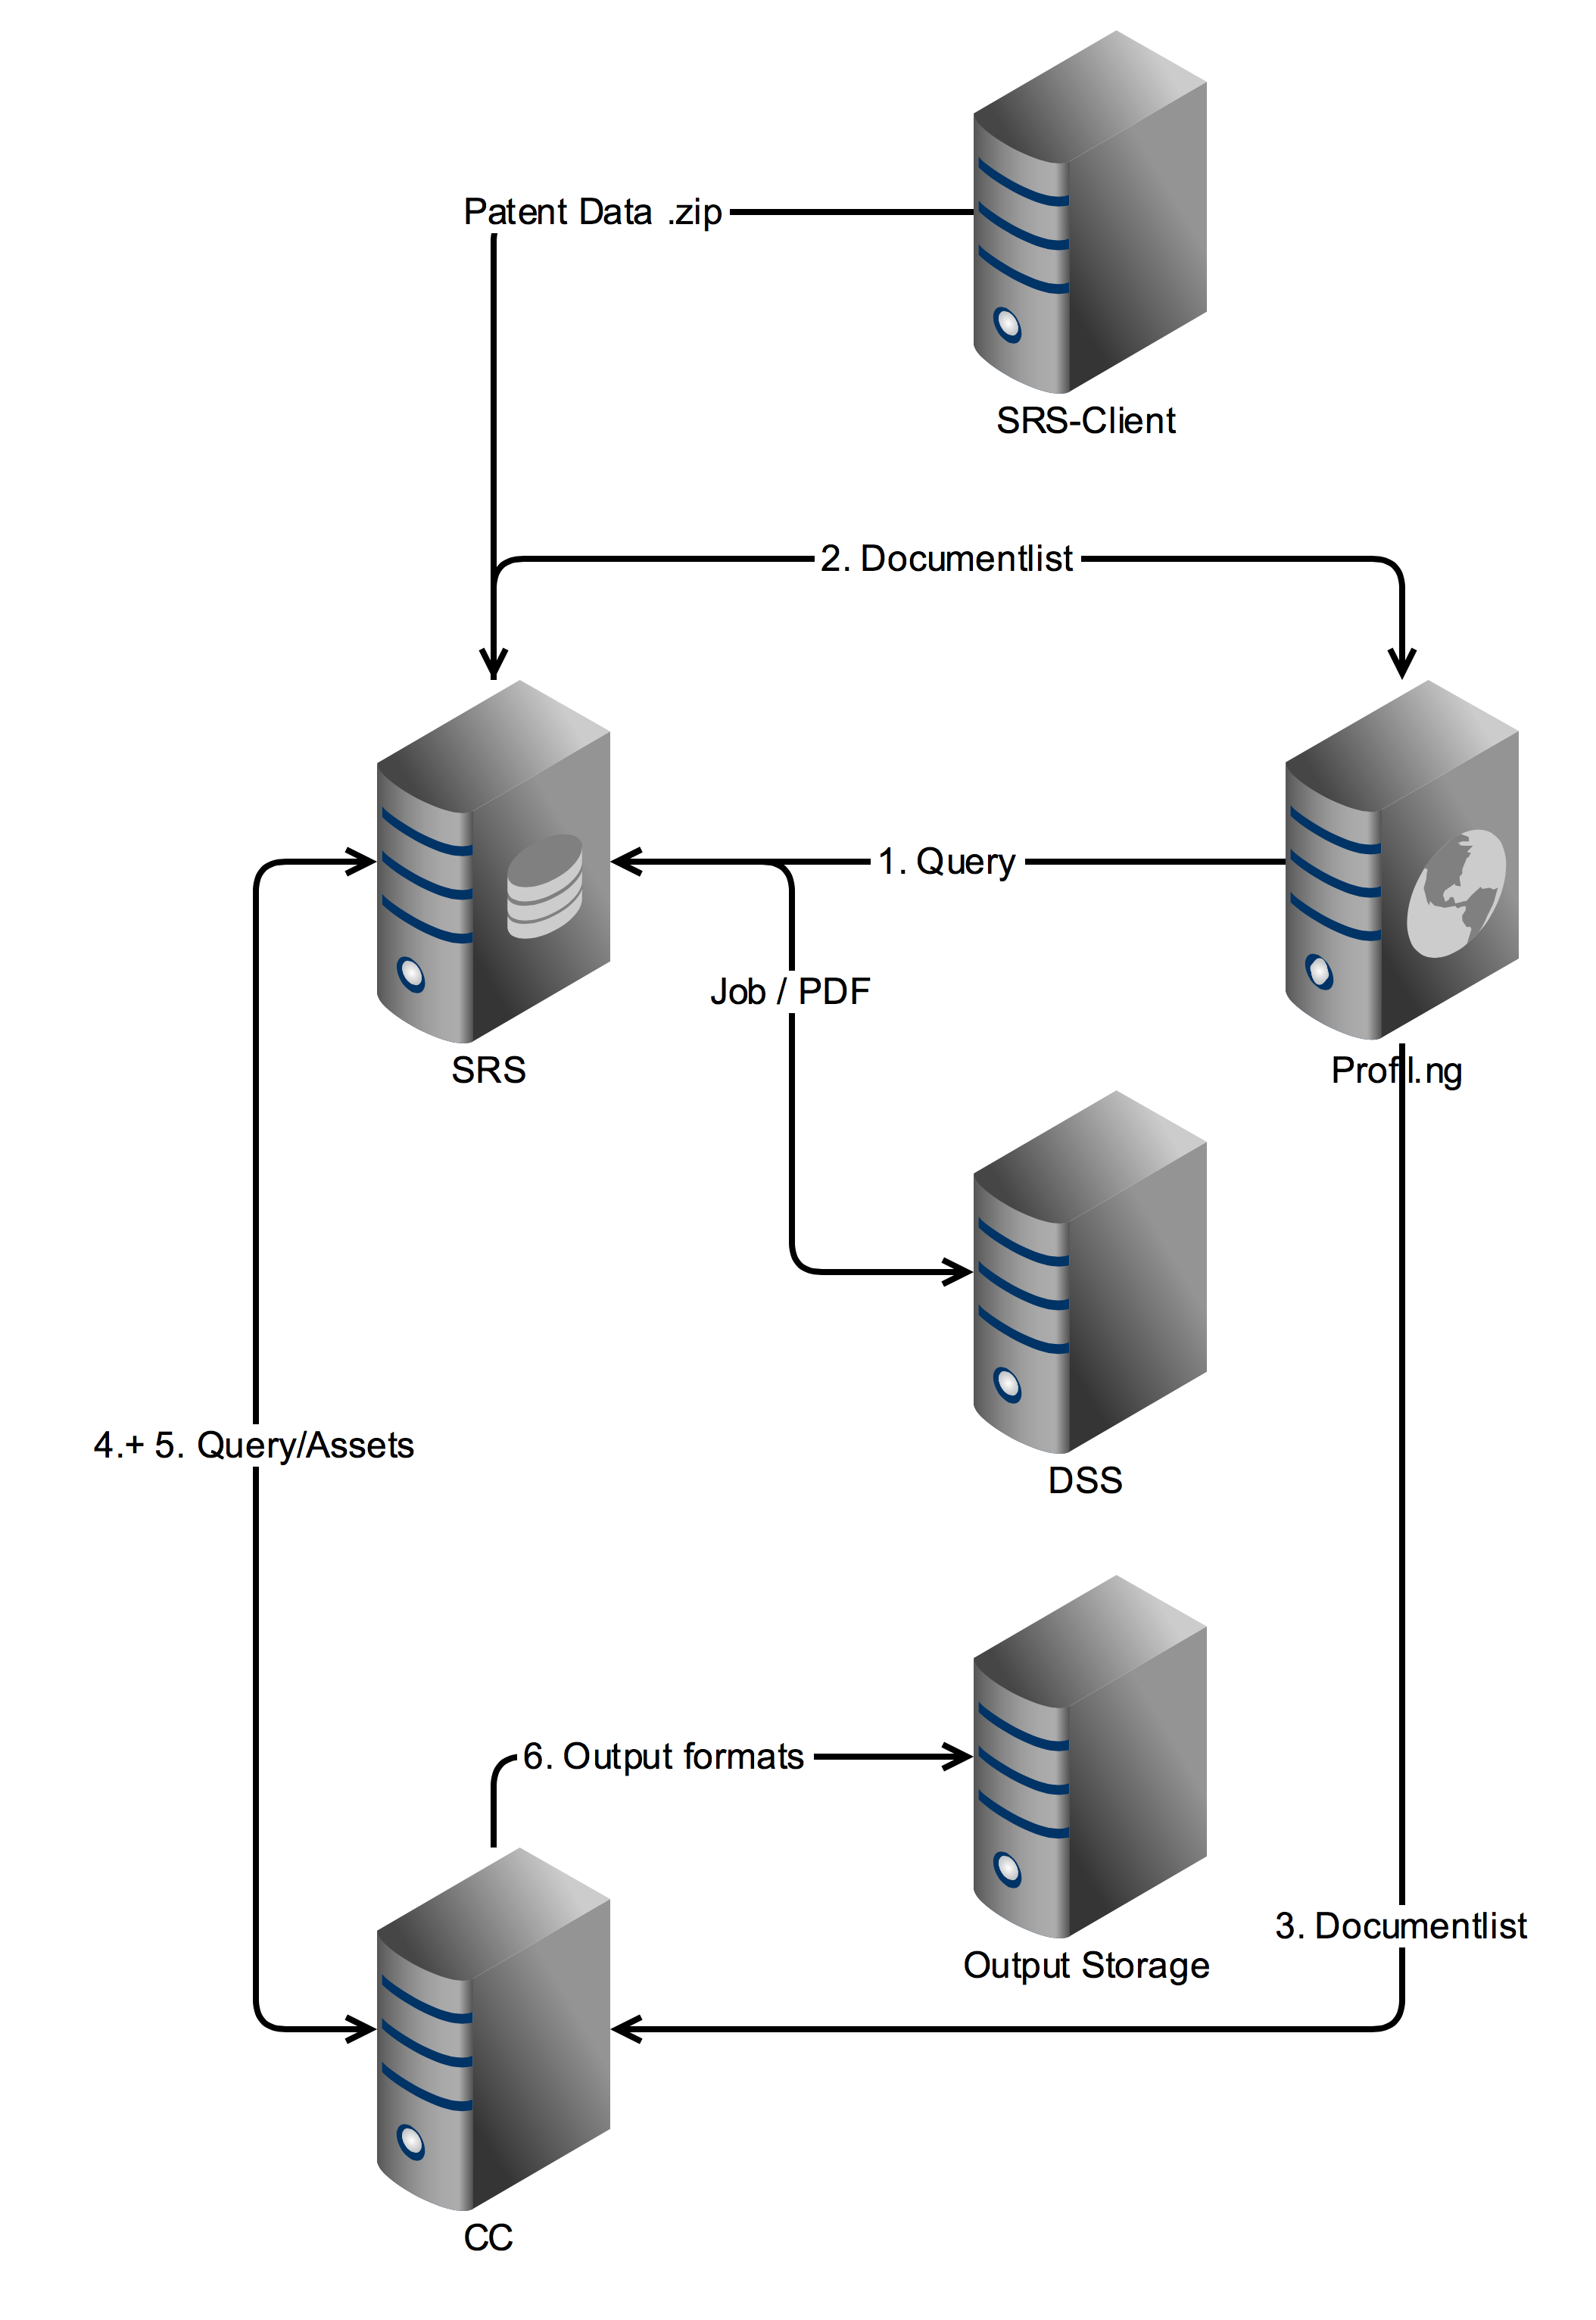
\includegraphics[width=0.9\textwidth]{gfx/dataflow-2.pdf}
  \caption{DEPAROM.NG Systemübersicht}
  \label{fig:DNGOverview}
\end{figure}

Die \autoref{fig:DNGOverview}, Seite \pageref{fig:DNGOverview} zeigt schematisch
das Zusammenspiel der verschiedenen Webdienste im DEPAROM.NG-Ökosystem.
Patentdaten werden als .zip-Dateien vom SRS-Client an den Simple Reference Store
übermittelt. Dieser verarbeitet die Patentdaten und speichert sie in
normalisierter Form ab. Wo notwendig, fordert der SRS beim DEPAROM Satz Service
(DSS) die Erstellung von Patentschriften im PDF-Format an.

Für die Produktion der Kundendatenträger sendet Profil.NG (PNG) eine Suchanfrage
an den SRS (1.). Dieser antwortet mit einer Dokumentliste, welche die
Dokument-IDs der gefundenen Patentdokumente enthält (2.). Anhand der
Dokumentliste erstellt PNG einen Job beim Collection Creator (3.), welcher die
notwendigen Artefakte zusammenträgt (4.+5.) und in einer Verzeichnisstruktur auf
dem Auslieferungsserver schreibt (6.), die dann auf einem Datenträger an den
Kunden übergeben werden.

\subsection{Simple Reference Store (SRS)}
\label{ch:fachlichesUmfeld:Teilsysteme:SRS}

Der sogenannte Simple Reference Store bildet den zentralen Datenspeicher von
DEPAROM.NG. Hier werden die Daten zu jedem Patentdokument gespeichert. Hierzu
gehören sowohl die originalen Dateien, wie sie von den jeweiligen Patentämtern
bezogen wurden, als auch normalisierte Daten im JSON und XML-Format. Das
normalisierte Format wird MTC-Format genannt. In \autoref{fig:SRSImport}, Seite
\pageref{fig:SRSImport} ist schematisch  der Datenstrom und die beteiligten
Softwarekomponenten aufgezeigt. Nachdem die Daten aus dem Patent-XML nach JSON
überführt wurden, werden auch die übrigen Artefakte (Zeichnungen, Faksimile)
extrahiert und auf einem Dateiserver abgelegt. SRS stellt auch diese Bild- und
PDF-Dateien bereit. Der Zugriff erfolgt über eine REST-Schnittstelle. Die
JSON-Formate werden in Elasticsearch gespeichert, indiziert und suchbar gemacht.

\begin{figure}[h]
  \includegraphics[width=0.9\textwidth]{gfx/srs-import.pdf}
  \caption{Datenstrom bei SRS-Import}
  \label{fig:SRSImport}
\end{figure}

SRS stellt auch eine Schnittstelle für Suchanfragen bereit, welche
Patentdokumente in konfigurierbaren Formaten und Detailgraden zurückliefert.

\subsection{DEPAROM Satz Service (DSS)}
\label{ch:fachlichesUmfeld:Teilsysteme:DSS}

Ein wichtiger Bestandteil der Patentinformationslieferungen aus DEPAROM.NG sind
die vollständigen Patentschriften im PDF-Format. Unglücklicherweise werden diese
nicht immer von den Patentämtern in der notwendigen Qualität geliefert. In
diesem Falle müssen die PDF-Dateien aus dem XML und den Bilddateien unter
Verwendung von XSL-FO erstellt werden. Der DSS übernimmt diese Aufgabe.

\subsection{DEPAROM Collection Creator (DCC)}
\label{ch:fachlichesUmfeld:Teilsysteme:DCC}

Der Dienst produziert Ausgabeformate, welche an Kunden für bestimmte
Dienstleistungen ausgeliefert werden. Derzeit produziert der DCC das für den
DEPAROM-Rechercheclient notwendige DVD-Format. Als Eingabedaten akzeptiert der
DCC Dokumentnummerlisten, anhand derer der Dienst die Patentdokumente
identifizieren kann, die in ein Ausgabeformat exportiert werden sollen.

\subsection{Profil.NG (PNG)}
\label{ch:fachlichesUmfeld:Teilsysteme:PNG}

Die Anwendung zur Steuerung des wöchentlichen Produktionsprozesses für den
Patentinformationsdienst DEPAROM Profil. PNG ist Gegenstand dieser
Bachelorarbeit. Sie soll die Operatoren befähigen, die
Patentinformationslieferungen zu produzieren und Abrechnungsdaten für die
Buchhaltung und Rechnungstellung zu generieren.

\cleardoublepage % Empty page before the start of the next part

\ctparttext{Der Hauptteil der vorliegenden Bachelorarbeit beschreibt die
Realisierung des in der Einleitung umrissenen Projekts. Es werden zunächst erste
Lösungsansätze diskutiert. Anschließend sollen die Lösungsansätze in Form von
Planung, Entwurf und Implementierung des Softwaresystems auf ihre
Realisierbarkeit geprüft werden.}

\part{Realisierung} % First part of the thesis
% Chapter 1

\chapter{Lösungsansätze} % Chapter title

\label{ch:Lösungsansätze} % For referencing the chapter elsewhere, use \autoref{ch:introduction}

%----------------------------------------------------------------------------------------

Im bestehenden System DEPAROM-Profil ist die sogenannte "`Profilanwendung"' die
zentrale Steuerungsanwendung für die Operatoren. Es handelt sich bei dieser
Anwendung um eine monolithische Anwendung mit grafischer Benutzeroberfläche, die
viele verschiedene Aufgaben erfüllt. Hierzu gehören auch Aufgaben, die nicht
direkt mit der Produktion der Patentinformationslieferungen zu tun haben, wie
beispielsweise der Import der Rohdaten, die Indexierung und die
Datenbankverwaltung. Hieraus resultiert eine schwere Wartbarkeit.

Die neue "`Profilanwendung"' mit der Bezeichnung "`Profil.NG"' soll einen enger
gefassten Scope erhalten. Sie soll ausschliesßlich verwaltende und steuernde
Aufgaben erfüllen. Die eigentliche Arbeit wird durch einzelnen Webdienste
verrichtet.

Folgende Probleme müssen vorrangig gelöst werden.

\section{Produktionsplan}
\label{ch:Lösungsansätze:Produktionsplan}

Die verschiedenen Suchaufträge müssen in regelmäßigen Abstanden durchgeführt
werden. Hierzu wurde bisher durch ein Perlscript eine Textdatei generiert,
welche die einzelnen Produktionsdaten für jede Kalenderwoche enthält. Das
Perlscript kann nur Produktionsdaten etwa 12 Monate im voraus generieren. Läuft
der aktuelle Produktionsplan aus, muss das Skript neu angestoßen werden, mit den
Parametern für den neuen Produktionszyklus. Wird dies vergessen, kommt es zu
Fehlerzustaänden, die nur durch Entwickler behoben werden können.

Um diesen Umstand zu umgehen, soll ein wochenbasierter Kalender implementiert
werden, welcher die Produktionsereignisse verwaltet, so dass die Operatoren sich
nicht mehr um den Produktionsplan kümmern müssen.

Die Verwaltung der sich wiederholenden Ereignisse ist niht ganz trivial und ich
möchte einige Lösungsideen diskutieren.

\subsection{Der berechnete Kalender}
\label{ch:Lösungsansätze:Produktionsplan:BerechneterKalender}

Um die Datenhaltung möglichst simpel zu halten, zog ich zunächst ein Modell in
betracht, bei dem nur die Kalenderwoche des Beginns der Patentüberwachung sowie
das Zeitintervall für die Wiederholung gespeichert würde. Mit diesen Daten wäre
es möglich für jede Kalenderwoche die fälligen Suchaufträge zu berechnen.

Dieses Modell funktioniert leider nur gut, wenn keine Unregelmäßigkeiten im
Zeitablauf vorkommen. Möchte man einzelne Ereignisse verschieben oder aussetzen,
müsste man Ausnahmeobjekte speichern und diese bei jedem Anzeigen des
Produktionsplans abrufen, um ggf. die Regelereignisse zu ignorieren. Mir
erschien diese Vorgehensweise als zu kompliziert. Zu dem müssen Metadaten zu den
Ereignissen gespeichert werden, und es muss möglich sein, bereits geschehene
Ereignisse zurückzusetzen, damit man eine fehlerbehaftete
Patentinformationslieferung erneut produzieren kann.

Da die Anforderungen das Modell des berechneten Kalenders übersteigen, und
ohnehin zu jedem Produktionsereignis weitere Daten gespeichert werden müssen
verwarf ich dieses Modell zugunsten eines Modells, das ich "Persistierter
Kalender" nenne.

\subsection{Der persistierte Kalender}
\label{ch:Lösungsansätze:Produktionsplan:PersistierteKalender}

Bei diesem Modell wird der Beginn der Patentüberwachung gespeichert und auch
jedes Produktionsereignis als eigenes Objekt. Dies ermöglicht das
Speichern zusätzlicher Metainformationen, die für jedes Ereignis individuell
sein können. Teil der Anforderung ist bspw. auch, dass Produktionsläufe
zurückgesetzt werden können. Dies ist z.B. dann erforderlich, wenn unbemerkt
fehlerhafte Eingangsdaten verarbeteitet wurden, oder wenn Patente von einem
Patentamt depubliziert werden.

Der Vorteil dieser Lösung liegt in seiner Flexibilität. Es ist nun möglich,
Produktionsläufe zu verschieben, zu löschen oder zurückzustellen und es können
beliebige Metadaten zu jedem Produktionslauf gespeichert werden.

Bei der Erstellung eines Suchauftrages müssen allerdings alle
Produktionsereignisse über den Überwachungszeitraum berechnet, erstellt und
gespeichert werden. Dies kann abhängig von Dauer und Häufigkeit der
Patentüberachung zu einer großen Zahl an Datenbankoerationen führen. Zudem ist
noch ungeklärt, wie mit Suchaufträgen umgegangen werden soll, die kein
Ablaufdatum besitzen.

Vermutlich wird es aber auf einen Algorhitmus hinauslaufen, der die
Produktionsereignisse zunächst für einen festgelegten Zeitraum im Voraus
erstellt (bspw. für 12 Monate). Im Modell der Produktionsereignisse wird es dann
eine Routine geben die prüft, ob noch Produktionsereignisse bevorstehen und ggf.
weitere 12 Monate mit Produktionsereignissen füllen.

\section{Interserverkommunikation}
\label{ch:Lösungsansatze:Interserverkommunikation}

Die Kommunikation mit anderen Diensten über ein Netzwerk ist eine völlig neue
Problematik, die beim bisherigen System nicht auftrat. Da DEPAROM.NG aus
verschiedenen Diensten mit fest definierten Aufgaben besteht, muss Profil.NG
alle Aufgaben delegieren, die außerhalb ihres Scopes liegen. Hierzu gehören u.a.
die Patentsuche und die Erstellung der Ausgabeformate.

Diese Aufgaben laufen asynchron ab und können einige Zeit in Anspruch nehmen. Es
wird also erforderlich sein, eine Methode zur Verwaltung dieser Aufgaben zu
entwickeln. Ein gangbarer Weg wäre es, eine Work Queue zu implementieren, in
der die einzelnen Jobobjekte abgearbeitet werden können. Darüber hinaus sollten
die Jobobjekte in der Datenbank persistiert werden, damit sie auch einen
Serverneustart überleben und die Produktionsvorgänge konsistent bleiben.

% Chapter 1

\chapter{Pflichtenheft} % Chapter title

\label{ch:Pflichtenheft} % For referencing the chapter elsewhere, use \autoref{ch:introduction} 

%----------------------------------------------------------------------------------------
Hier werden die Grundlagen für das zu entwickelnde Softwaresystem definiert.
Zwar noch aus fachtechnischer Sicht werden hier die Anforderungen an das
geplante Softwaresystem in möglichst formaler Form spezifiziert. Es sollen hier
keine Lösungen präsentiert werden, sondern möglichst präzise die Anforderungen
(Sollkonzept) an das geplante Softwaresystem mit seinen Schnittstellen,
Informationsflüssen und Systemfunktionen dokumentiert werden. Verwendete
Methoden können z.B. SA, SADT, Petri-Netze oder andere sein.

Das Ergebnis ist ein für die Systementwicklung verwendbares Pflichtenheft. Über
Art und Umfang des Pflichtenhefts sollten Sie mit Ihrem Betreuer sprechen.

% Chapter 1

\chapter{Systementwurf} % Chapter title

\label{ch:Systementwurf} % For referencing the chapter elsewhere, use \autoref{ch:introduction}

%----------------------------------------------------------------------------------------

Zur besseren Einordnung von Profil.NG in das Gesamtsystem DEPAROM.NG sei hier
nochmals auf die  Systemübersicht (\autoref{fig:DNGOverview}, Seite
\pageref{fig:DNGOverview}) verwiesen.

Im folgenden Teil sollen die für Profil.NG verwendeten Technologien, die
Motivation hinter deren Verwendung und spezifische Entwurfsprobleme in Bezug auf
den Technologiestack näher beleuchtet werden.

\section{Systemarchitektur}

Das System Profil.NG besteht aus

\begin{itemize}
  \item{einer Clientkomponente}
  \item{einer Serverkomponente}
  \item{einer Datenbankkomponente}
\end{itemize}

Die Clientkomponente wird die Aufgaben der Benutzerschnittstelle übernehmen. Sie
soll als Fat-Client konzipiert in einem modernen Webbrowser laufen. Aufgrund der
Betriebsumgebung in einem Webbrowser ist die gewählte Programmiersprache
natürlicherweise JavaScript.

Die Kommunikation zwischen dem Client und dem Server wird über Websockets
ablaufen. Das Protokoll für die Datenübertragung wird das Distributed Data
Protcol \cite{ddp} sein.

Die Serverkomponente beherbergt die Geschäftslogik und ist für die Kommunikation
mit der Datenbank zuständig. Auch das Serverprogramm wird in JavaScript
geschrieben.

Das Datenbanksystem wird MongoDB sein, eine nichtrelationale, dokumentbasierte
Datenbank. Sie akzeptiert JSON-Dokumente, das Datenaustauschformat von
JavaScript, als Eingabedaten und eignet sich daher gut für ein System, welches
mehrheitlich in JavaScript geschrieben ist.

\begin{figure}[h]
  \includegraphics[width=0.9\textwidth]{gfx/meteor_architektur.pdf}
  \caption{Vereinfachte Meteor Systemarchitektur nach \cite{meteor-architecture}}
  \label{fig:MeteorArchitektur}
\end{figure}

\subsection{Programmiersprache und Plattform}

Die Entwicklungsplattform wird Meteor sein, eine komplett in JavaScript
geschriebene Plattform für die Entwicklung von Webanwendungen. Meteor stellt
eine isomorphe API für Client- und Serverentwicklung bereit. Meteor folgt sieben
Designprinzipien \cite{meteor-7}, die interessierten Entwicklern eine Umgebung
für effizientes und schnelles Entwickeln von Webanwendungen ermöglichen soll.

\begin{quotation}

  \begin{description}

    \item[Datenübertragung]{Meteor schickt kein HTML über das Netzwerk, sondern
    nur Daten. Der Client rendert diese Daten dann}

    \item[Eine Sprache]{Sowohl Client-, als auch Serverkomponente werden in
    JavaScript geschrieben}

    \item[Datenbank überall]{Die Datenbank kann auf Client- und auf Serverseite
    mit den gleichen Methoden manipuliert werden.}

    \item[Verzögerungskompensierung]{Auf der Clientseite werden Daten
    vorgespeichert und Datenbankoperationen simuliert, um eine verzögerungsfreie
    Benutzererfahrung zu ermöglichen.}

    \item[Reaktivität über alle Schichten]{Mit Meteor ist Echtzeit der Standard.
    Alle Schichten, von der Datenbank bis zu den Templates, aktualisieren sich
    selbständig.}

    \item[Nutze das Ökosystem]{Meteor lässt sich einfach mit bestehenden
    Bibliotheken und Frameworks integrieren.}

    \item[Einfach bedeutet produktiv]{Die beste Art, etwas einfach aussehen zu
    lassen ist, etwas tatsächlich einfach zu machen. Die Hauptfunktionen von
    Meteor stellen einfache APIs bereit.}

  \end{description}

\end{quotation}

Die Wahl viel auf Meteor, da ich mir insbesondere aufgrund der Einsprachigkeit,
der Isomorphie und der vollständigen Reaktivität Effizienzsteigerungen bei der
Entwicklung verspreche.

Zudem bietet Meteor die Möglichkeit, das Programm für verschiedene
Zielplattformen (derzeit Node.js, Android und iOS) zu kompilieren. So wird das
Bedienen der unterstützten Plattformen stark vereinfacht.

Meteor wurde auch deshalb ausgewählt, um Erfahrungen mit der Plattform zu
sammeln, so dass sich MTC ggf. auch strategisch auf diese Plattform stützen kann
und auch zukünftige Projekte mit dieser Technologie realisieren kann.

\subsection{Benutzerschnittstelle}

Blaze

\subsection{Datenbanksystem}

MongoDB

\section{Drei-Schicht-Architektur nach Meteor}

???

\section{Fachklassenmodell}

Aus den fachlichen Anforderungen in \autoref{ch:Pflichtenheft}
(\pageref{ch:Pflichtenheft}) konnte ich ein Aktivitätsmodell ableiten, das ich
in Form eines Aktivitätsdiagramms (\autoref{fig:PNGActivity}, Seite
\pageref{fig:PNGActivity}) abgebildet habe.

\begin{figure}[H]
  \includegraphics[width=0.9\textwidth]{gfx/activity.pdf}
  \caption{Profil.NG - Aktivitätsmodell}
  \label{fig:PNGActivity}
\end{figure}

Die in diesem Diagramm wiederkehrenden Begriffe "`Kunde"', "`Monitoring"',
"`Query"' bildeten die Basis für das Fachklassenmodell
(\autoref{fig:PNGFachklassen}, Seite \pageref{fig:PNGFachklassen}).7

Hierbei ist anzumerken, dass in einer früheren Version die Klasse "`Occurance"'
noch nicht existierte. Als während der Analyse der Geschäftsprozesse jedoch die
Anforderung ermittelt wurde, dass Produktionsläufe einzelner
Überwachungsaufträge rückgängig gemacht oder für eine spätere Produktion
zurückgestellt werden sollten, wurde schnell klar, dass jedes
Produktionsereignis einzeln behandelt werden muss und sich das Konzept des
Berechneten Kalenders in
\autoref{ch:Lösungsansätze:Produktionsplan:BerechneterKalender} (Seite
\pageref{ch:Lösungsansätze:Produktionsplan:BerechneterKalender}) als nicht
ausreichend für die gestellten Anforderungen erwies.

Die Klasse "`DeliveredDoc"' leitete ich aus der Anforderung ab, dass keine
Patentdokumente doppelt an einen Kunden ausgeliefert werden dürfen. Deshalb
werden Objekte gespeichert, die ausgelieferte Dokumente repräsentieren und die
eindeutig einem bestimmten Monitoring zugeordnet werden.

\begin{figure}[H]
  \includegraphics[width=0.9\textwidth]{gfx/fachklassen.pdf}
  \caption{Profil.NG - Fachklassenmodell}
  \label{fig:PNGFachklassen}
\end{figure}

\section{Sequenzdiagramme}

Im folgenden werden Sequenzdiagramme angegeben, welche Funktionalitäten abbilden,
die nicht von Meteor-Standardfunktionen (wie z.B. Login/Logout) abgedeckt sind.

\subsection{[03] Kunde anlegen}

\begin{figure}[H]
  \includegraphics[width=0.9\textwidth]{gfx/03-kunde-anlegen.pdf}
  \caption{Anwendungsfall 03: Kunde anlegen}
  \label{fig:AF03}
\end{figure}

\subsection{[04] Kunde bearbeiten}

\begin{figure}[H]
  \includegraphics[width=0.9\textwidth]{gfx/04-kunde-bearbeiten.pdf}
  \caption{Anwendungsfall 04: Kunde bearbeiten}
  \label{fig:AF04}
\end{figure}

\subsection{[05] Überwachungsauftrag erstellen}

\begin{figure}[H]
  \includegraphics[width=0.9\textwidth]{gfx/05-uberwachungsauftrag-erstellen.pdf}
  \caption{Anwendungsfall 05: Überwachungsauftrag erstellen}
  \label{fig:AF05}
\end{figure}

\subsection{[06] Suchprofil erstellen}

\begin{figure}[H]
  \includegraphics[width=0.9\textwidth]{gfx/06-suchprofil-erstellen.pdf}
  \caption{Anwendungsfall 03: Suchprofil erstellen}
  \label{fig:AF06}
\end{figure}

\subsection{[07] Trefferlisten erstellen}

\begin{figure}[H]
  \includegraphics[width=0.9\textwidth]{gfx/07-trefferlisten-erstellen.pdf}
  \caption{Anwendungsfall 07: Trefferlisten erstellen}
  \label{fig:AF07}
\end{figure}

\subsection{[08] Trefferlisten anzeigen}

\begin{figure}[H]
  \includegraphics[width=0.9\textwidth]{gfx/08-trefferlisten-anzeigen.pdf}
  \caption{Anwendungsfall 08: Trefferlisten anzeigen}
  \label{fig:AF08}
\end{figure}

\subsection{[09] Ausgabeformate erstellen}

\begin{figure}[H]
  \includegraphics[width=0.9\textwidth]{gfx/09-ausgabeformate-erstellen.pdf}
  \caption{Anwendungsfall 09: Ausgabeformate erstellen}
  \label{fig:AF09}
\end{figure}

\subsection{[10.1] Produktion zurücksetzen (Trefferlisten)}

\begin{figure}[H]
  \includegraphics[width=0.9\textwidth]{gfx/10-1-produktion-reset-hitlist.pdf}
  \caption{Anwendungsfall 10.1: Produktion zurücksetzen (Trefferlisten)}
  \label{fig:AF10-1}
\end{figure}

\subsection{[10.2] Produktion zurücksetzen (Ausgabeformate)}

\begin{figure}[H]
  \includegraphics[width=0.9\textwidth]{gfx/10-2-produktion-reset-output.pdf}
  \caption{Anwendungsfall 10.2: Produktion zurücksetzen (Ausgabeformate)}
  \label{fig:AF10-2}
\end{figure}

% Chapter 1

\chapter{Implementierung} % Chapter title

\label{ch:implementierung}

%-------------------------------------------------------------------------------

Die Implementierung erfolgte auf Basis der Plattform Meteor. Da Meteor die aus
anderen Plattformen wie Java Enterprise, ASP.net oder Python/Django bekannte
Trennung von Client und Server auflöst, war es nötig in der
Implementierunsarbeit neue Wege zu finden, um eine saubere Softwarearchitektur
zu ermöglichen. Die  wesentlichen Maßnahmen hierzu, sowie die generelle
Vorgehensweise sollen in diesem Kapitel diskutiert werden.

Der Stand der Implementierung zum Zeitpunkt der Erstellung dieser Arbeit ist
unvollständig. Die Analyse der Anforderungen sowie der Entwurf des Systems wurde
immer wieder verzögert. Behinderungsfaktoren waren zum Einen
Terminschwierigkeiten mit den beteiligten Produktverantwortlichen, zum anderen
zunächst unscharfe und später wechselnde Anforderungen an das System. Dies
führte schlussendlich dazu, dass für die Implementierung nur etwa vier Wochen zu
Verfügung standen.

\section{Meteorspezifika}

Die Meteorplattform kommt mit einem eigenen Buildsystem, welches den Quellcode
packt, minimiert und für die Integration auf einem Node.js-Server bereit macht.
Damit dieses System wie erwartet funktioniert muss der Entwickler einigen
Konventionen bei der Wahl der Verzeichnisse beachten, da bestimmte Verzeichnisse
nur auf dem Client, nur auf dem Server oder aber auf beiden Seiten ausgeliefert
werden. Zudem werden die Verzeichnisse in einer bestimmten Reihenfolge geladen,
was bei Codefragmenten wichtig werden kann, die von einander Abhängig sind.

\begin{description}
  \item[server]{Wird nur an den Server ausgeliefert}
  \item[client]{Wird nur an de Client ausgeliefert}
  \item[tests]{Wird nur in der Testkonfiguration ausgeliefert}
  \item[lib]{Wird in einer Verzeichnisebene zuerst geladen}
\end{description}

Alle übrigen Verzeichnisse werden auf Client und Server ausgeliefert. Dateien
und Verzeichnisse werden, beginnend mit der tiefsten Verzeichnisebene, in
alphabetischer Reihenfolge geladen.

Ich folgte bei meiner Implementierung den Konventionen aus dem "`Unofficial
Meteor FAQ"' \cite{meteor-faq}, welche hier kurz als Beispielverzeichnisbaum
dargestellt werden soll.

\begin{lstlisting}[caption=Empfohlene Verzeichnisstruktur für Meteorprojekte \cite{meteor-faq}, language=sh]
lib/                       # <- any common code for client/server.
lib/environment.js         # <- general configuration
lib/methods.js             # <- Meteor.method definitions
lib/external               # <- common code from someone else
## Note that js files in lib folders are loaded before other js files.

collections/               # <- definitions of collections and methods on them (could be models/)

client/lib                 # <- client specific libraries (also loaded first)
client/lib/environment.js  # <- configuration of any client side packages
client/lib/helpers         # <- any helpers (handlebars or otherwise) that are used often in view files

client/application.js      # <- subscriptions, basic Meteor.startup code.
client/index.html          # <- toplevel html
client/index.js            # <- and its JS
client/views/<page>.html   # <- the templates specific to a single page
client/views/<page>.js     # <- and the JS to hook it up
client/views/<type>/       # <- if you find you have a lot of views of the same object type
client/stylesheets/        # <- css / styl / less files

server/publications.js     # <- Meteor.publish definitions
server/lib/environment.js  # <- configuration of server side packages

public/                    # <- static files, such as images, that are served directly.

tests/                     # <- unit test files (won't be loaded on client or server)
\end{lstlisting}

\section{Vorgehensweise}

Um die Reihenfolge der zu implementierenden Anforderungen zu bestimmen, nahm ich
die erstellten User Stories und sortierte sie zunächst nach den wichtigsten bzw.
am schwierigsten zu implementierenden User Stories. Die mir am wichtigsten
erscheinende User Story ist \nameref{ch:SystemEntwurf:07} (Seite
\pageref{ch:SystemEntwurf:07}), da die Trefferliste den eigentlichen Mehrwert
der Dienstleistung Deparom-Profil und somit den zentralen Use Case darstellt.

Damit diese User Story realisiert werden kann identifizierte ich andere User
Stories, die als Vorraussetzung gelten.

\begin{enumerate}
  \item{\nameref{ch:SystemEntwurf:03}, Seite \pageref{ch:SystemEntwurf:03}}
  \item{\nameref{ch:SystemEntwurf:04}, Seite \pageref{ch:SystemEntwurf:04}}
  \item{\nameref{ch:SystemEntwurf:05}, Seite \pageref{ch:SystemEntwurf:05}}
  \item{\nameref{ch:SystemEntwurf:06}, Seite \pageref{ch:SystemEntwurf:06}}
\end{enumerate}

Bei der eigentlichen Implementierungsarbeit folgte ich den Prinzipien der
testgetriebenen Entwicklung \cite{tdd}, bei der zunächst ein programmatischer
Test die gewünschte Funktionalität prüft. Natürlicherweise scheitert dieser
Test, da die notwendige Implementierung fehlt.

Anschließend wird die fehlende Implementierung erarbeitet, bis der Test
erfolgreich verläuft.

Man beginnt nun mit dem nächsten Test und macht immer so weiter.

\subsection{Testgetriebene Entwicklung mit Meteor}

Für die testgetriebene Entwicklung stellt Meteor ein Testframework namens
Velocity \cite{velocity} bereit. Das Framework nutzt die Reaktivität von Meteor,
überwacht den Quellcode und lässt alle vorhandenen Tests ablaufen, sobald eine
geänderte Quelldatei gespeichert wird. Hierdurch kann sich der Entwickler auf
die Implementierung konzentrieren, da das Neuladen und Testen der Anwendung vom
Framework automatisch durchgeführt wird. Als Entwickler muss man nur noch die
Testergebnisse überprüfen.

Velocity unterstützt verschiedene Testbibliotheken. Ich verwendete Jasmine 2.1
\cite{jasmine}, eine Bibliothek die Unit und Integration Tests ermöglicht.
Jasmine ermöglicht das Schreiben von Tests sowohl für den Client, als auch für
den Server.

\section{Tests}

Dem Testen der Anwendung wurde viel Aufmerksamkeit und Entwicklungszeit
gewidmet. Aus diesem Grunde sollen einige Tests im Detail besprochen werden, um
die Besonderheiten beim Testen von Meteor-Applikationen aufzuzeigen.

\subsection{Unit Tests}

Bei den Tests konzentrierte ich mich vor allem auf die das Fachklassenmodell.
Eine vollständige Abdeckung meines Quellcodes mit Tests ist zwar erstrebenswert,
im Hinblick auf die Zeitbeschränkungen jedoch nicht zielführend.

Exemplarisch soll hier die Unit-Testsuite für die Customers-Klasse diskutiert
werden.

\lstinputlisting[caption=Unit Tests für Customers-Klasse]{/Users/timjagodzinski/src/don.ng/profil-ng/tests/jasmine/server/unit/customerModelSpec.js}

Ab Zeile 7 im obigen Listing wird mit der Funktion \textit{spyOn} ein sog. Spy
definiert. Ein Spy überwacht ein Objekt und protokolliert die Zugriffe auf das
Objekt. Auf das Protokoll kann zugegriffen werden, um das Verhalten der
Anwendung zu testen. Darüber hinaus ist es möglich, Funktionen zu definieren,
die aufgerufen werden, wenn ein überwachtes Objekt auf eine bestimmte Art und
Weise aufgerufen wird.

Diese Funktionalität wird im obigen Listing verwendet, um den Callback des
Aufrufs von Meteor.call() zu simulieren. Dies wird durch die Verkettung des
\textit{spyOn}-Aufrufs mit den Methoden \textit{.and.callFake()} erreicht, wobei
\textit{callFake} als Parameter die gewünschte Funktion entgegennimmt.

In der vorliegenden Implementierung wird nur der \textit{callback} mit den
Argumenten \textit{null}, \textit{1} aufgerufen. So wird simuliert, dass die
Meteor.method \textit{customerSave} ein leeres \textit{error}-Objekt und die ID
des neu hinzugefügten Customer-Objekts zurückgibt.

Die folgenden Zeilen bis Zeile 20 definieren ein Testdatenobjekt, anhand dem die
Konstruktorfunktion in Zeile 24 aufgerufen wird.

Ab Zeile 26 wird dann überprüft, ob der Inhalt der Felder des
\textit{customer}-Objekts denen des Testdatenobjekts entspricht. Dabei
referenziere ich auf das Testdatenobjekt und vermeide Verwendung von Literalen,
um die Vergleiche zu machen. Dies soll Fehler durch Tippfehler vermeiden.

Eine frühere Version dieses Tests nutzte zum Prüfen der Feldwerte des
\textit{customer}-Objekts Literale. Dabei unterlief mir ein Tippfehler und der
Test schlug fehl. Daraufhin führte ich eine Refakturierung auf die oben
abgebildete Version durch und vermied es auch in den weiteren Tests, Literale
zur Prüfung zu verwenden.

\subsection{Integration Tests}

Um das Zusammenspiel der einzelnen Komponenten der Anwendung zu testen, bedient
man sich der Integrationstests. Diese werden verwendet, um die Schnittstellen
der verwendeten Module zu testen, aber auch um das Zusammenspiel von Front- und
Backend zu testen, sowie das Verhalten der Clientapplikation in Bezug auf
Anwenderinteraktion.

Bei der Implementierungsarbeit für Profil.NG nutzte ich Integrationstests, um die
Routenkonfiguration zu testen. Hierbei war mir besonders wichtig sicherzustellen,
dass geschützte Routen nur für angemeldete Benutzer sichtbar sind.

Darüber hinaus habe ich die Beschaffenheit von Templates, insbesondere von
Formularen überprüft, sowie das Eventhandling auf den Routen.

Exemplarisch sollen hier die Tests für die Routen und Controller diskutiert
werden, welche für das Erstellen und Bearbeiten von Customer-Objekten zuständig
sind.

Da Integrationstests auf einer echten Instanz der Anwendung laufen, ist es
notwendig Testdaten vorzubereiten, die von der Anwendung verwendet werden
können. Insbesondere ist es nötig, ein Benutzerkonto anzugeben, damit sich der
virtuelle Anwender bei der Applikation authentifizieren kann.

Zu diesem Zweck wird eine Funktion definiert, welche aufgerufen wird, wenn die
Anwendung gestartet in der Testkonfiguration gestartet wird. Im folgenden
Listing ist zu sehen, wie des Testbenutzerkonto in der Funktion
\textit{loadDefaultFixtures()} definiert wird.

\lstinputlisting[firstline=50,caption=Fixtures für Integrationstests]{/Users/timjagodzinski/src/don.ng/profil-ng/tests/jasmine/server/integration/fixtures/database-fixture.js}

Die Testsuite für die Route, die für das Hinzufügen von Customer-Objekten
verwendet wird soll im Folgenden beschrieben werden.

\lstinputlisting[caption=Integrationstest für Kunde-Speichern-Formular]{/Users/timjagodzinski/src/don.ng/profil-ng/tests/jasmine/client/integration/customers/customersAddSpec.js}

Als erstes wird geprüft, ob die geforderte Route unter dem geforderten Namen
\textit{customersAdd} existiert und ob diese zur URL \textit{/customers/add}
führt.

\begin{lstlisting}[caption=Test auf Existenz der Route 'customersAdd']
  describe("route", function() {
    it("should be at path '/customers/add'", function() {
      expect(Router.routes["customersAdd"].path()).toBe(
        "/customers/add");
    });
  });
\end{lstlisting}

Dieser Test ist wichtig, um die generelle Routenkonfiguration der Anwendung zu
validieren. Falsche Routen, Pfade oder geänderte Routen sind häufige
Fehlerquellen in meiner Entwicklungsarbeit gewesen. Insbesondere bei steigender
Komplexität der Anwendung ist eine einwandfreie Routenkonfiguration wichtig, um
Doppelbelegungen von URLs oder die falsche Verwendung von Routen zu vermeiden.

Der eigentliche Test wird in der Testsuite \textit{view} beschrieben. Anzumerken ist hier
zunächst der Block mit den Aufrufen von \textit{beforeEach()} und \textit{afterEach} der im
folgenden Listing dargestellt ist.

\begin{lstlisting}[caption=Vor- und Nachtestkonfiguration]
  beforeEach(function(done) {
      Meteor.loginWithPassword("ops@profil.ng", "start1234",
        function(
          error) {
          done();
        });
    });

    beforeEach(function(done) {
      Router.go("/customers/add");
      Tracker.afterFlush(done);
    });

    beforeEach(waitForRouter);

    afterEach(function(done) {
      Meteor.logout(function() {
        done();
      });
    });
\end{lstlisting}

Die \textit{beforEach()}-Aufrufe werden vor jedem Test ausgeführt. Sie enthalten
für gewöhnlich Konfiguration und Abläufe, die für die kommenden Test wichtig
sind. In der vorliegenden Implementierung meldet sich der Testclient mit den
Nutzerdaten an, die in der Fixture schon definiert wurden. Anschließend wird der
Router aufgerufen und ändert die URL auf den vorher getesten Wert. Mit
\textit{beforeEach(waitForRouter);} wartet der Testclient darauf, dass die Seite
vollständig geladen ist, um  sicherzustellen dass der DOM vollstaändig ist. So
wird gewährleitet, dass die folgenden Tests, welche nach bestimmten
DOM-Elementen suchen auch erfolgreich ablaufen können.

Der Rest der Testsuite befasst sich mit dem eigenlichen Formular und überprüft,
ob alle erforderlichen Formularfelder und Schaltflächen vorhanden sind.

Mit Integrationstests kann auch das Verhalten der Anwendung bei Benutzerinteraktion
getestet werden. Hierfür soll zur Demonstration ein Auszug aus der Testsuite des
Controllers für die Route \textit{customersAdd} dienen.

\begin{lstlisting}[caption=Test des Verhaltens bei Benutzereingabe]
  it("should save the form contents to a new customer object on submit",
		function() {
			var customer;

			fillForm();
			spyOn(Customers, "insert");

			$(".ui.form.segment").form().submit();
			expect(Customers.insert).toHaveBeenCalled();
			expect(Customers.insert).not.toThrow();
		});
\end{lstlisting}

Mit der Hilfsfunktion \textit{fillForm()} wird zunächst das HTML-Formular mit
Daten gefüllt. Dies geschieht unter Zuhilfname der DOM-Manipulationsbibliothek
jQuery. Anschließend wird ein Submit-Event mittels jQuery ausgelöst, der
wiederum die Datenbankoperation zum Speichern des Customer-Objekts auslösen
soll. Das verhalten wird mit den beiden \textit{expect()}-Aufrufen überprüft.

Bei dieser Art Test ist es wichtig, das gewünschte Ergebnis abzutesten. In
diesem Fall der Aufruf der Insert-Methode auf der Customers-Collection. Der Weg
dort hin, also die eigentliche Implementierung sollte nicht abgetestet werden.
Dies würde dazu führen, dass bei Änderungen in der Implementierung der Test ggf.
scheitert, obwohl die Implementierung immer noch das gewünschte Ergebnis
liefert. Man spricht in diesem Fall von sogenannten "`brittle"' Tests
\cite{brittle-tests}.

\section{Fachklassen}

Sowohl auf Client als auch auf dem Server existiert das eigentliche Model in
Form einer Konstruktorfunktion, welche das jeweilige Model beschreibt. Objekte
die aus diesen Konstruktorfunktion erstellt werden rufen ihrerseits
Meteor.methods auf, wenn sie Datenbankoperationen veranlassen sollen. Diese
werden zum Zwecke der leichteren Zuordnung direkt neben den
Konstruktorfunktionen, also in der gleichen Datei definiert.

Die verschiedenen Modelle der Geschäftslogik sind im Verzeichnis \textit{models}
gesammelt.

Die Modelle enthalten vor allem CRUD-Operationen und sollen wegen ihrer
Einfachheit hier nicht näher erlautert werden.

\section{Publications und Subscriptions}

Meteor verwendet einen besonderen Mechanismus, um Daten vom Server zu Beziehen.
Da Meteor nicht dem klassischen Zyklus von Anfrage und Antwort des
HTTP-Protokolls folgt, sondern Daten per Websockets direkt an den Client
überträgt ist es erforderlich, Endpunkte auf dem Server zu definieren, an denen
sich ein Client anmelden kann, um Daten zu beziehen. Diese Endpunkte werden bei
Meteor \textit{Publications} genannt. Mittels einer Publication wird eine
Funktion  definiert welche einen oder mehrere Datenbankcursors zurückliefert,
welche dann vom Client genutzt werden können, um Daten abzurufen.

Die Publications für das Customer-Modell sehen wie folgt aus:

\lstinputlisting[caption=Definition der Publication für die Customers-Collection]{/Users/timjagodzinski/src/don.ng/profil-ng/server/publications/customersPublications.js}

Ein Client kann sich an diese Publications anmelden. Dafür muss der Methode
\textit{Meteor.subscribe()} der Name der Publication, sowie ggf. nötige
Parameter übergeben werden. Als Rückgabewert erhält man einen
Subscription-Handle, mittels dem man dann die eigentlichen Daten beziehen kann.

Dieses Modell verleitet zunächst dazu, sehr weit gefasste Publications zu
schreiben, damit alle Daten, die zu einem Benutzer gehören auf den Client
synchronisiert werden, und dieser mit allen Daten lokal Arbeiten kann. Bei kleineren
Datenmengen ist dies noch ein gangbarer Weg. Aber bei großen Datenmengen wird diese
Vorgehensweise zu einem Performanceproblem.

Auf der Clientseite kann der initiale Aufruf der Anwendung mit einer sehr langen
Ladezeit verbunden sein, da erst alle Daten synchronisiert sein müssen, bevor
die Anwendung gestartet werden kann. Auf der Serverseite führen weit gefasste
Publications zu einem sehr großen Arbeitsspeicherverbrauch, da der
Node.js-Server alle Daten im Speicher behält, die in einer Pulication an einen
bestimmten Client ausgeliefert wurden. Dies ist notwendig, damit der Server bei
Änderungen in der Datenbank einen Abgleich ausführen kann, damit nur ein
Datenpatch und nicht der komplette Datensatz an den Client geschickt werden
müssen.

Aus diesem Grunde gilt der Grundsatz der Datensparsamkeit beim Entwurf von
Publications und beim Einsatz von Subscriptions. In der Implementierung der
Routecontroller wurde deshalb darauf geachtet, nur Subscriptions anzumelden, die
für die aktuelle Route relevant sind. Siehe dazu folgendes Listing.

\begin{lstlisting}[caption=Auszug aus Routecontroller für Route 'customers']
Router.route('/customers', function() {
  	this.render('Customers');
  }, {
  	name: 'customers',
  	waitOn: function() {
  		Meteor.subscribe("getCustomersList");
  	},
  	data: function() {
  		return {
  			customers: Customers.find().fetch()
  		};
  	}
});
\end{lstlisting}

\cleardoublepage % Empty page before the start of the next part

\ctparttext{Preamble für Auswertungsteil} % Text on the Part 2 page describing the content in Part 2
\part{Ergebnisse} % First part of the thesis
% Chapter 1

\chapter{Bedienungsanleitung} % Chapter title

\label{ch:bedienungsanleitung} % For referencing the chapter elsewhere, use \autoref{ch:introduction}

%----------------------------------------------------------------------------------------

\section{Installationsvorraussetzungen}

Für die Installation der Entwicklerversion wird benötigt:

\begin{description}
  \item[Betriebssystem]{Mac OSX oder Linux}
  \item[curl]{Um das Installationsscript zu beziehen und auszuführen}
  \item[Internetverbindung]{Die Installation ist nur über das Internet möglich}
\end{description}

Die Installation einer Produktivumgebung ist komplexer und soll nicht Gegenstand
dieser Arbeit sein.

\section{Installation und Start}

Installieren Sie die Meteorplattform mittels folgendem Shell-Befehl:

\begin{verbatim}
  $> curl https://install.meteor.com/ | sh
\end{verbatim}

Kopieren sie das Verzeichnis \textit{Quellcode/profil-ng} von dem beiliegenden
Datenräger auf ein beliebiges Festplattenlaufwerk ihres Computers und wechseln
in das betreffende Verzeichnis.

Starten Sie die Anwendung mit dem Befehl

\begin{verbatim}
  $> meteor
\end{verbatim}

Meteor installiert jetzt alle Abhängigkeiten und startet anschließend den
Entwicklungsserver. Die Webanwendung ist unter der URL
\textit{http://localhost:3000} über einen Webbrowser erreichbar.

\section{Unterstützte Webbrowser}

Folgende Webbrowser wurden getestet und offiziell unterstützt:

\begin{itemize}
  \item{Google Chrome}
  \item{Apple Safari}
\end{itemize}

Firefox wurde zwar nicht getestet, es ist aber wahrscheinlich, dass
Profil.NG problemlos mit Firefox zusammenarbeitet.

Microsoft Internet Explorer wurde in keiner Version getestet. Es werden
keinerlei Garantien für die Verwendung übernommen.


\section{Benutzerhandbuch}

Profil.NG erlaubt die Verwaltung der Produktionsabläufe für DEPAROM-Profil,
sowie der für die Produktion relevanten Stammdaten der Kunden. Hierzu gehören
Kundendaten, Überwachungsaufträge und Queries.

\subsection{Vor dem Erstbetrieb}

Da alle Funktionen hinter einem Login verborgen sind, muss zunächst ein
Benutzerkonto angelegt werden. Den Link zum Registrierungsformular finden Sie
unterhalb des Anmeldeformulars.

\begin{figure}[H]
  \includegraphics[width=0.9\textwidth]{gfx/login-register.pdf}
  \caption{Link zum Registrierungsformular}
  \label{fig:login-register}
\end{figure}

Füllen Sie das Registrierungsformular aus und klicken auf die Schaltfläche
\textit{Register Now!}. Ein Benutzerkonto wird für Sie angelegt und Sie werden
augenblicklich mit selbigem angemeldet.

\begin{figure}[H]
  \includegraphics[width=0.9\textwidth]{gfx/register-form.pdf}
  \caption{Registrierungsformular}
  \label{fig:register-form}
\end{figure}

\subsection{Kunde anlegen}

Klicken Sie in der Navigationsleiste auf die Schaltfläche \textit{Manage
customers}. Es erscheint eine Übersicht der im System befindlichen Kundenkonten.

\begin{figure}[H]
  \includegraphics[width=0.9\textwidth]{gfx/add-customer.pdf}
  \caption{Schaltfläche 'Add customer'}
  \label{fig:add-customer}
\end{figure}

Klicken Sie auf die Schaltfläche \textit{Add customer}, um das Formular zum
Erstellen eines neuen Kunden zu öffnen. Füllen Sie das Formular aus. Mit einem
Stern markierte Felder sind Pflichtfelder. Bitte lassen Sie diese nich leer.
Sind Sie mit Ihrer Eingabe zufrieden, klicken Sie auf die Schaltfläche
\textit{Save customer}

\begin{figure}[H]
  \includegraphics[width=0.9\textwidth]{gfx/add-customer-form.pdf}
  \caption{Formular für das Erstellen eines neuen Kunden}
  \label{fig:add-customer-form}
\end{figure}

\subsection{Überwachungsauftrag anlegen}

Klicken Sie in der Navigationsleiste auf die Schaltfläche \textit{Manage
customers}. Es erscheint eine Übersicht der im System befindlichen Kundenkonten.

Klicken Sie auf den Namen eines Kunden, um die Ansicht zum Bearbeiten des Kunden
zu öffnen. Siehe \autoref{fig:add-customer}, Seite \pageref{fig:add-customer}.

Scrollen Sie in der Ansicht zum Bearbeiten des Kunden nach unten, bis die
Schaltfläche \textit{Add monitoring} erscheint. Klicken Sie auf diese
Schaltfläche.

\begin{figure}[H]
  \includegraphics[width=0.9\textwidth]{gfx/add-monitoring.pdf}
  \caption{Schaltfläche 'Add monitoring'}
  \label{fig:add-monitoring}
\end{figure}

Füllen Sie das Formular zum Anlegen eines neuen Überwachungsauftrags aus.
Klicken Sie auf die Schaltfläche \textit{Save monitoring}, wenn Sie mit ihren
Eingaben zufrieden sind.

\begin{figure}[H]
  \includegraphics[width=0.9\textwidth]{gfx/add-monitoring-form.pdf}
  \caption{Formular für das Erstellen eines neuen Überwachungsauftrags}
  \label{fig:add-monitoring-form}
\end{figure}

\subsection{Suchanfrage anlegen}

Klicken Sie in der Navigationsleiste auf die Schaltfläche \textit{Manage
customers}. Es erscheint eine Übersicht der im System befindlichen Kundenkonten.

Klicken Sie auf den Namen eines Kunden, um die Ansicht zum Bearbeiten des Kunden
zu öffnen. Siehe \autoref{fig:add-customer}, Seite \pageref{fig:add-customer}.

Klicken Sie auf die \textit{Profile \#} eines Monitorings, um die Ansicht zum
Bearbeiten des Monitorings zu öffnen. Siehe \autoref{fig:add-monitoring}, Seite
\pageref{fig:add-monitoring}.

Scrollen Sie in der Ansicht zum Bearbeiten des Monitorings nach unten, bis die
Schaltfläche \textit{Add query} erscheint. Klicken Sie auf diese Schaltfläche.

\begin{figure}[H]
  \includegraphics[width=0.9\textwidth]{gfx/add-query.pdf}
  \caption{Schaltfläche 'Add query'}
  \label{fig:add-query}
\end{figure}

Füllen Sie das Formular zum Anlegen eines neuen Queries aus.
Klicken Sie auf die Schaltfläche \textit{Save query}, wenn Sie mit ihren
Eingaben zufrieden sind.

\begin{figure}[H]
  \includegraphics[width=0.9\textwidth]{gfx/add-query-form.pdf}
  \caption{Formular für das Erstellen eines neuen Query}
  \label{fig:add-query-form}
\end{figure}

% Chapter 1

\chapter{Zusammenfassung und Ausblick} % Chapter title

\label{ch:zusammenfassungUndAusblick} % For referencing the chapter elsewhere, use \autoref{ch:introduction}

%----------------------------------------------------------------------------------------


Im Verlauf dieser Bachelorarbeit konnten die Anforderungen an das System
\textit{Profil.NG} aus dem Vorgängersystem \textit{Profilanwendung} estrahiert,
bereinigt und formuliert werden. Aus den Anforderungen  ließ sich ein für die
Implementierung verwendbar Software-Entwurf ableiten, welcher für die
Entwicklung des vorliegenden Prototyps benutzt wurde.

Die Analyse- und Entwurfsphase fiel dabei überraschend groß aus. Es war
schwierig, die Anforderungen aus dem Vorgängersystem in einer ausreichenden
Abstraktion herauszulösen und für Profil.NG zu formulieren. Erschwerend kamen
Faktoren hinzu, die nicht im Bereich des Software-Engineering liegen. So waren
die für die Ermittlung der Geschäftsprozesse nötigen Personen nicht immer
zeitnah zu sprechen und es war zum Teil schwierig ihnen die Wichtigkeit ihrer
Rolle begreiflich zu machen. Hieraus resultierten zunächst unscharfe
Anforderungen, die sich im weiteren Verlauf des Projekts auch änderten. Hieraus
resultierten Verzögerungen, die darin resultierten, dass verhältnismäßig wenig
Implementierungszeit zu Verfügung stand.

Das gewählte Entwicklungsverfahren der testgetriebenen Entwicklung erwies sich
zugleich als herausragend nützliches Werkzeug und als stärkste Bremse während
der Implementierungsphase. Die besondere Denkweise bei der testgetriebenen
Entwicklung und die geringe Erfahrung sowohl mit der Testbibliothek Jasmine als
auch in der testgetriebenen Entwicklung im Allgemeinen und mit Meteor im
speziellen erwiesen sich immer wieder als Implementierungsbremsen, da hier viel
Forschungsarbeit geleistet werden musste. Da man bei der Implementierung aber
gezwungen wird, sich zunächst über den gewünschten Effekt Gedanken zu machen und
nicht gleich in Implementierungsdetails verrennt, erlangt man ein besseres
Verständnis über die logische Problematik der Implementierung. Zudem kann man
sich in der testgetriebenen Entwicklung relativ sicher sein, keine
Implementierungsdetails vergessen zu haben, sobald alle Tests erfolgreich
verlaufen.

In Ermangelung von ausreichend Implementierungszeit ist vor allem noch die
Kommunitation mit den anderen Webdiensten im DEPAROM.NG-Gesamtsystem eine
ungelöste Aufgabe. Meteor liefert mit \textit{http} eine Bibliothek, die für
exakt diese Aufgabe entwickelt wurde. Eine Realisierung anhand von \textit{http}
scheint daher keine besonders schwierige Aufgabe.

Ein Problem ganz anderer Art ist die Schemavalidierung. Ein weitgehend
ungelöstes Problem im Meteor-Ökosystem ist die Validierung von Eingabedaten
gegen ein Dokumentschema. Durch die Definition solcher Schemata wäre es möglich,
solche Validierungen in einer standadisierten Art und Weise durchzuführen. Auch
wäre es möglich, Formulare für CRUD-Operationen programmatisch aus solchen
Schemata zu generieren. Während der Bearbeitungszeit für diese Arbeit stieß ich
leider erst recht spät auf eine Bibliothek, welche die Definition einfacher
Schemata ermöglicht. Die Verwendung selbiger vermied ich, da mein Zeitplan
ohnehin schon sehr knapp bemessen war.

Für die Zukunft soll eine Schemadefinition in jedem Fall hinzugefügt werden.

Im weiteren Verlauf des Projekts Profil.NG außerhalb dieser Bachelorarbeit soll
die testgetriebene Entwicklung in jedem Falle weitergeführt werden. Die
Anwendung wird für die Generierung von mehreren hunderttausend Euro Umsatz im
Jahre die zentrale Rolle spielen, weshalb eine reibungslose Weiterentwicklung zu
gewaährleisten ist. Ich ziehe auch in Erwägung die vorhandenen Testkategorien
Unit- und Integrationstests noch um Akzeptanztests zu erweitern. Als mögliche
Technologien zur Realisierung sehe ich hier die Frameworks Cucumber oder
Nightwatch. Eine genauere Evaluierung der beiden Technologien sollte die Eignung
für Meteor allerdings zuvor feststellen.

\cleardoublepage % Empty page before the start of the next part

%----------------------------------------------------------------------------------------
%	THESIS CONTENT - APPENDICES
%----------------------------------------------------------------------------------------

\appendix

\part{Anhang} % New part of the thesis for the appendix

% Appendix X

\chapter{Code Listings}

%----------------------------------------------------------------------------------------

% Content begins here

Als Software-Spezialist können Sie selbstverständlich hervorragend
programmieren. Das wird vorausgesetzt und sollte nicht die primäre Leistung
eines Informatikers sein. Dennoch macht es oft Sinn dem interessierten Leser
Einblick in den Source-Code zu gewähren. Hier bietet es sich an,
Programm-Listings in Form eines extra gebundenen Anhangs zur Diplomarbeit zu
dokumentieren. Weniger an Programmierdetails Interessierte können sich dann
"unbeschwerter" der eigentlichen Arbeit widmen.
 % Appendix A
%% Appendix X

\chapter{Appendix Title}

%----------------------------------------------------------------------------------------

% Content begins here % Appendix B - empty template

%----------------------------------------------------------------------------------------
%	POST-CONTENT THESIS PAGES
%----------------------------------------------------------------------------------------

\cleardoublepage% Bibliography

\label{app:bibliography} % Reference the bibliography elsewhere with \autoref{app:bibliography}

\manualmark
\markboth{\spacedlowsmallcaps{\bibname}}{\spacedlowsmallcaps{\bibname}}
\refstepcounter{dummy}

\addtocontents{toc}{\protect\vspace{\beforebibskip}} % Place the bibliography slightly below the rest of the document content in the table of contents
\addcontentsline{toc}{chapter}{\tocEntry{\bibname}}

\bibliographystyle{abbrvdin}

\bibliography{Bibliography}
 % Bibliography

\cleardoublepage% Declaration

\refstepcounter{dummy}
\pdfbookmark[0]{Software}{software} % Bookmark name visible in a PDF viewer

\chapter*{Software} % Applied software section text

Für die Erstellung dieser Arbeit wurden eine Vielzahl von Programmen verwendet.
Im Folgenden möchte ich versuchen, eine Auflistung der wichtigsten zu liefern.

\thispagestyle{empty}

\begin{description}
  \item[Atom] \hfill \\
  Der Texteditor mit dem diese Arbeit erstellt und der Quellcode geschrieben
  wurde. http://www.atom.io
  \item[MacTex-2014] \hfill \\
  Die \LaTeX\-Distribution für Mac OS X, mit der diese Arbeit gesetzt wurde.
  https://tug.org/mactex/
  \item[Meteor-Plattform] \hfill \\
  Die Plattform für Real-Time-Webanwendungen, mit der Profil.NG entwickelt
  wurde. https://www.meteor.com
  \item[Jasmine] \hfill \\
  Die JavaScript-Bibliothek für Unit- und Integrationstests, mit der die
  Testsuite für Profil.NG geschrieben wurde. http://jasmine.github.io
  \item[Velocity] \hfill \\
  Das Testframework, welches für die testgetriebene Entwicklung von Profil.NG
  verwendet wurde. http://velocity.meteor.com
  \item[Semantic-UI] \hfill \\
  Das CSS-Framework, mit dem die Benutzeroberfläche für Profil.NG erstellt
  wurde. http://semantic-ui.com
  \item[Safari] \hfill \\
  Einer der beiden Webbrowser, mit denen Profil.NG hauptsächlich entwickelt
  wurde. Einige der Abbildungen wurden mit Safari von SVG nach PDF konvertiert.
  https://www.apple.com/de/safari/
  \item[Chrome] \hfill \\
  Der andere Webbrowser, mit dem Profil.NG entwickelt wurde. Über Chrome wurden
  vor allem die Unit- und Integrationstests abgewickelt.
  https://www.google.de/chrome/browser/desktop/
  \item[Gliffy] \hfill \\
  Die Webanwendung, mit der einige der Abbildungen in dieser Arbeit erstellt
  wurden. https://www.gliffy.com
  \item[StarUML] \hfill \\
  Das UML-Entwurfswerkzeug, mit dem die UML-Diagramme erstellt wurden.
  http://staruml.io
  \item[Adobe Acrobat] \hfill \\
  Das PDF-Werkzeug von Adobe. Es wurde zum Zuschneiden einiger PDF-Zeichnungen
  benutzt. http://www.adobe.com/de/products/acrobat.html
\end{description}
 % Software used to produce the thesis and implementation

\cleardoublepage% Colophon (a brief description of publication or production notes relevant to the edition)

\pagestyle{empty}

\hfill

\vfill

\pdfbookmark[0]{Kolophon}{kolophon}

\section*{Kolophon}

Dieses Dokument wurde mit dem LaTeX-Template \texttt{classicthesis} von Andr\'e
Miede gesetzt. Der Stil wurde durch das Buch über Typographie von Robert
Bringhurst mit dem Titel ``\emph{The Elements of Typographic Style}''.
\texttt{classicthesis} inspiriert. Er ist für \LaTeX\ und \mLyX verfügbar:

\begin{center}
\url{http://code.google.com/p/classicthesis/}
\end{center}

\noindent Anwender, die mit \texttt{classicthesis} zufrieden sind, senden dem
Autor für gewöhnlich eine Postkarte. Eine Sammlung der bisher eingesandten
Postkarten ist hier zu finden:

\begin{center}
\url{http://postcards.miede.de/}
\end{center}

\bigskip

\noindent\finalVersionString
 % Colophon

\cleardoublepage% Declaration

\refstepcounter{dummy}
\pdfbookmark[0]{Declaration}{declaration} % Bookmark name visible in a PDF viewer

\chapter*{Declaration} % Declaration section text

\thispagestyle{empty}

Ich erkläre hiermit, dass die vorliegende Arbeit von mir selbständig erarbeitet
wurde. Es wurden nur erlaubte Hilfsmittel verwendet. Die Stellen in dieser
Arbeit, die in Wortlaut oder Sinn anderen Quellen entnommen wurden, habe ich
entsprechend mit Angabe der Quelle gekennzeichnet. Dies gilt auch für
Internetquellen, welche ich in Kopie im Anahang oder auf dem beiliegenden
Datenträger hinterlegt habe.

\bigskip
 
\noindent\textit{\myLocation, \myTime}

\smallskip

\begin{flushright}
\begin{tabular}{m{5cm}}
\\ \hline
\centering\myName, \today \\
\end{tabular}
\end{flushright}
 % Declaration

%----------------------------------------------------------------------------------------

\end{document}
